\documentclass[runningheads]{llncs}

\usepackage[T1]{fontenc}
\usepackage[utf8]{inputenc}
\usepackage{graphicx}
\usepackage{booktabs}
\usepackage{amsmath,amssymb}
\usepackage{array}
\usepackage{hyperref}

\graphicspath{{../outputs/}}

\title{Detection-Probability-Oriented Waveform Co-Optimization for ISAC Power Allocation: A \texttt{UMi\_NLOS} Case Study}

\author{Anonymous Author}
\institute{Prepared from the ISAC Power Allocation project repository}

\begin{document}
\maketitle

\begin{abstract}
This paper replaces the usual SNR-based sensing metric in an integrated sensing and communication (ISAC) power-allocation problem with detection probability, so that waveform shaping becomes a direct design variable rather than a side detail. We study a weighted rate--detection formulation over a time-varying OFDM channel and optimize both power and a normalized waveform profile. The experiments use a \texttt{UMi\_NLOS} scenario with false-alarm probability $P_{\mathrm{fa}}=10^{-3}$, which defines the detection regime for the reported $P_d$ values. In the Pareto study, Grey Wolf Optimizer (GWO) spans the tradeoff from a sensing-focused point with $P_d=0.892$ at 10.70 bps/Hz to a communication-focused point with 22.76 bps/Hz and $P_d=0.212$. Compared with water-filling, which reaches 22.50 bps/Hz but only $P_d=0.114$, the proposed formulation keeps nearly the same rate while almost doubling detection probability at the rate-focused end, and it reaches a much stronger sensing point at the opposite end. This suggests that detection-aware waveform co-optimization gives a more useful ISAC tradeoff than power-only allocation.
\keywords{ISAC \and detection probability \and waveform co-optimization \and UMi\_NLOS \and Pareto analysis}
\end{abstract}

\section{Introduction}
Integrated sensing and communication (ISAC) tries to use the same transmission resources for both data transfer and sensing. For a detection-oriented sensing task, probability of detection is usually a better measure than sensing SNR alone. This paper therefore studies a detection-probability-centered ISAC problem instead of an SNR-centered one.

The work is deliberately framed as a case study. It does not claim to replace all detector design or all channel models. Instead, it asks a narrower question: in a realistic but still manageable \texttt{UMi\_NLOS} setting, which optimization method gives the best sensing-communication tradeoff when detection probability and waveform shaping are included?

The main contributions are:
\begin{itemize}
  \item a simple detection-probability objective that can be used directly in optimization,
  \item a normalized waveform profile that is optimized together with power,
  \item a comparison of several search algorithms on the same channel sequence,
  \item a Pareto-style view of the tradeoff between rate and sensing quality,
  \item a clear discussion of what the model does and does not include.
\end{itemize}

\section{Related Work and Scope}
ISAC has been studied from many angles, including fundamental limits, waveform design, and system-level tradeoffs \cite{liu2022isacsurvey,ouyang2023mi}. A consistent lesson from that literature is that the sensing metric must match the task. If the task is detection, then probability of detection is more meaningful than a proxy such as sensing SNR.

Waveform design is also a common theme in OFDM-based ISAC. Prior work has shown that waveform shaping can change the sensing--communication balance in a real way \cite{liyanarachchi2021waveforms}. This paper follows that idea, but keeps the model simple enough to focus on optimization behavior rather than on a very detailed radar signal chain.

The channel side of ISAC also matters. Standard channel descriptions such as 3GPP TR 38.901 motivate scenario-based studies instead of generic fading only \cite{3gpp38901}. That is why this paper uses \texttt{UMi\_NLOS} and a time-varying channel sequence.

The scope is intentionally limited:
\begin{itemize}
  \item one target return is modeled on the sensing side,
  \item clutter and multi-target effects are not modeled,
  \item the static study uses one representative snapshot,
  \item the paper compares optimization methods, not detector implementations.
\end{itemize}

\section{System Model}
We consider an OFDM system with 32 subcarriers and a time-varying channel sequence of 20 CSI snapshots in the \texttt{UMi\_NLOS} scenario. The channel includes path loss, shadowing, multipath delay spread, and Doppler variation. Communication and sensing use separate effective channel responses.

The representative snapshot in Figure~\ref{fig:channel} is clearly frequency selective, which is what makes joint power and waveform shaping useful in this setting.

\subsection{Waveform coupling (W3)}
The waveform profile $\mathbf{w}$ is a normalized per-subcarrier shaping profile. It is not an antenna beamformer because the model does not include array geometry. Instead, $\mathbf{w}$ is a simple spectral weighting vector that changes how strongly each subcarrier contributes to the communication and sensing branches.

We apply waveform shaping by raising each per-subcarrier weight to an exponent. Let $w_{\min}>0$ be a small floor value used for numerical stability. The communication rate is
\begin{equation}
R(\mathbf{p},\mathbf{w}) = \sum_{k=1}^{K} \log_2\!\left(1 + \frac{p_k\, g_{\mathrm{comm},k}\,\bigl(\max(w_k, w_{\min})\bigr)^{\beta_c}}{N_0}\right),
\label{eq:rate}
\end{equation}
and the sensing SNR proxy is
\begin{equation}
\mathrm{SNR}_{\mathrm{sense}}(\mathbf{p},\mathbf{w}) =
\frac{\sum_{k=1}^{K} p_k\, g_{\mathrm{sense},k}\,\bigl(\max(w_k, w_{\min})\bigr)^{\beta_s}}{K\,N_0}.
\label{eq:sensing_snr}
\end{equation}
Here $N_0$ is the (per-subcarrier) noise power, and $g_{\mathrm{comm},k}$ and $g_{\mathrm{sense},k}$ are the effective communication and sensing gains at subcarrier $k$.

The exponents $\beta_c$ and $\beta_s$ control how strongly waveform shaping affects communication and sensing. In our default setting, $\beta_c=0.15$ and $\beta_s=1.0$; we also use $w_{\min}=10^{-6}$. When waveform co-optimization is disabled, $\mathbf{w}$ is fixed to the flat profile $w_k=1$.

The waveform constraints are:
\begin{equation}
\sum_{k=1}^{K} w_k = K,\qquad w_k \ge w_{\min}\ \ \forall k,
\end{equation}
and power is constrained by a total budget with optional per-subcarrier caps.

\subsection{Detection probability mapping (W1)}
The sensing side uses a simple single-target, round-trip return model. An effective sensing SNR is first computed via \eqref{eq:sensing_snr}, then mapped to probability of detection using a Gaussian-tail approximation (so the paper is fully reproducible).

Let $Q(\cdot)$ be the standard Gaussian tail function, i.e., $Q(x)=1-\Phi(x)$. For a fixed false-alarm probability $P_{\mathrm{fa}}$, define the threshold
\begin{equation}
\eta = Q^{-1}(P_{\mathrm{fa}}) = \Phi^{-1}(1-P_{\mathrm{fa}}),
\end{equation}
where $\Phi(\cdot)$ is the standard Gaussian CDF.
We then apply an integration gain $G_{\mathrm{int}}$ (a tunable modeling constant) and compute
\begin{equation}
P_d = Q\!\left(\eta - \sqrt{2\,G_{\mathrm{int}}\,\mathrm{SNR}_{\mathrm{sense}}(\mathbf{p},\mathbf{w})}\right).
\label{eq:pd_mapping}
\end{equation}
This form follows standard Gaussian detection models used to relate an effective SNR to a tail probability \cite{kay_detection,richards_radar}. In the reported experiments we use $P_{\mathrm{fa}}=10^{-3}$ and $G_{\mathrm{int}}=0.02$. We treat $G_{\mathrm{int}}$ as a modeling knob that controls how quickly $P_d$ rises with sensing SNR; it is not presented as a detector-derived constant.

The objective is
\begin{equation}
J(\mathbf{p}, \mathbf{w}) = \alpha R(\mathbf{p}, \mathbf{w}) + (1-\alpha)\gamma U_{\mathrm{sense}},
\end{equation}
where $U_{\mathrm{sense}} = P_d$ in the default mode and $\gamma$ is a scaling factor used to keep the sensing term on a comparable numerical scale to the rate term. In all reported results, $\gamma=10$.

\subsection{Interpretation in plain language}
The waveform profile $\mathbf{w}$ can be read as a ``spectrum emphasis'' vector. If $\mathbf{w}$ is flat, all subcarriers contribute equally. If $\mathbf{w}$ is non-flat, some subcarriers are emphasized more than others, which lets the optimizer steer the design toward sensing-favorable or communication-favorable frequency regions.

\subsection{What is simplified}
The sensing model is simplified on purpose. It uses a single effective target return and does not include clutter, extended targets, or a separate noise-clutter covariance model. The paper should therefore be read as a benchmark study for detection-aware resource allocation, not as a final radar processing chain.

\begin{figure}[t]
\centering
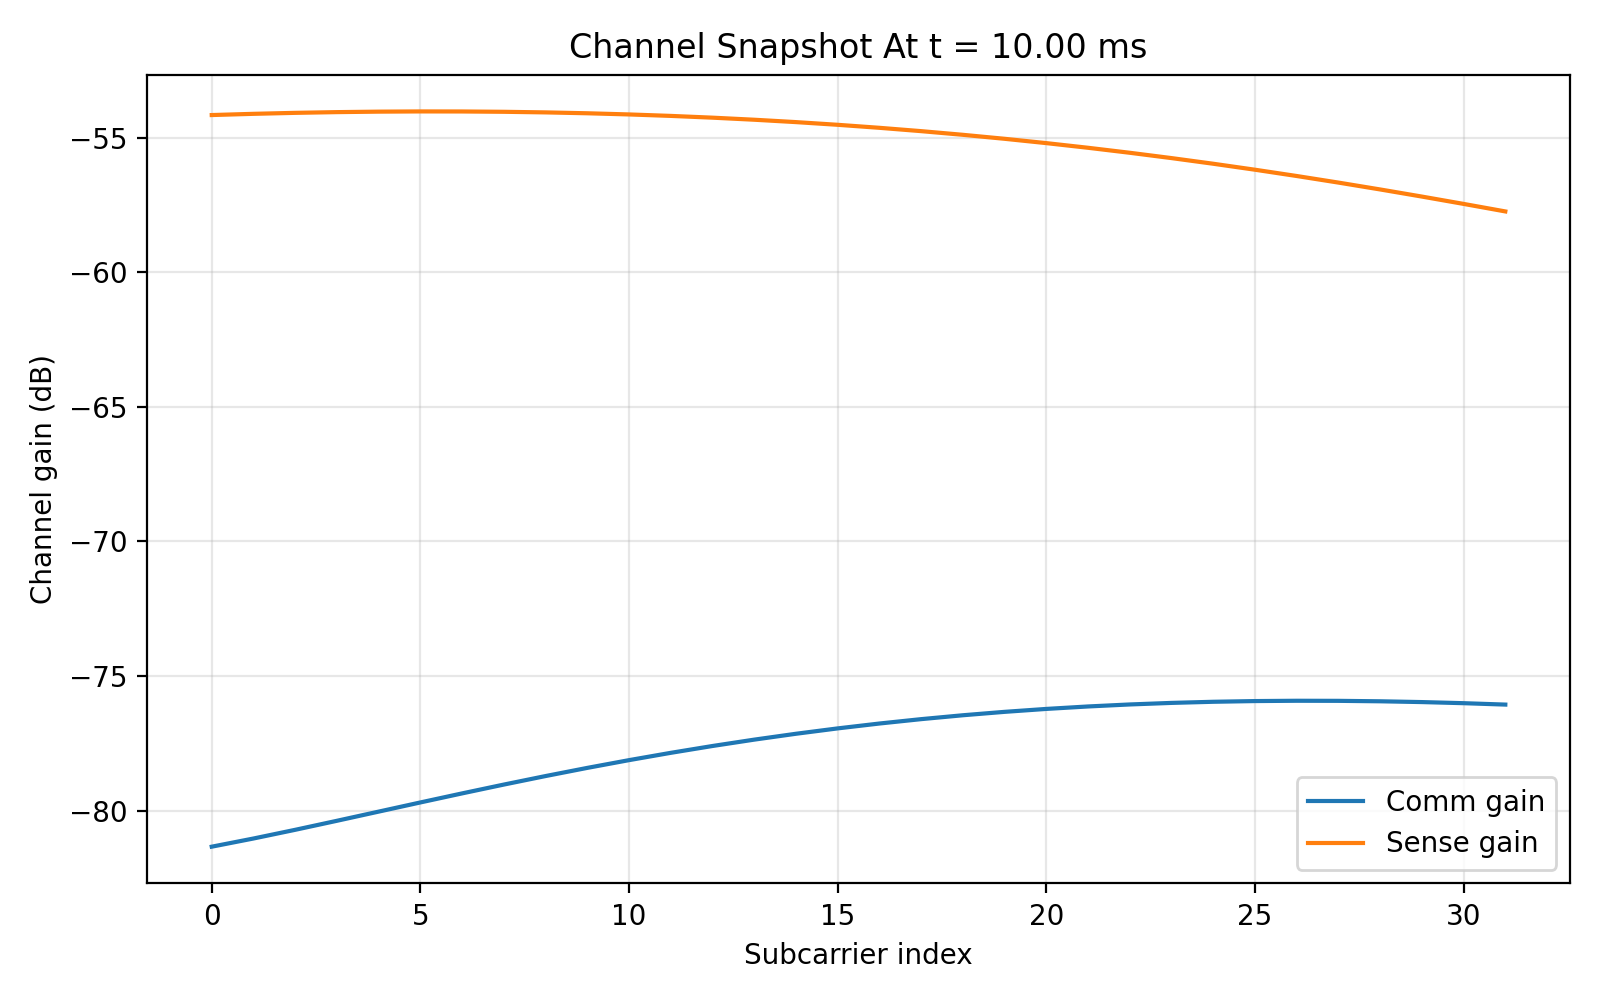
\includegraphics[width=0.82\textwidth]{channel_snapshot.png}
\caption{Representative \texttt{UMi\_NLOS} channel snapshot used in the static study.}
\label{fig:channel}
\end{figure}

\section{Method and Evaluation Protocol}
The same problem instance is given to every algorithm. This keeps the comparison fair and makes the results easier to read. The methods are compared in three ways:
\begin{itemize}
  \item a single representative snapshot,
  \item a dynamic sequence of 20 channel updates,
  \item a Pareto-style sweep over the weighted objective.
\end{itemize}

\begin{table}[t]
\centering
\caption{Key system and objective parameters used throughout the case study.}
\label{tab:params}
\small
\begin{tabular}{lc}
\toprule
Parameter & Value \\
\midrule
Scenario & \texttt{UMi\_NLOS} \\
Subcarriers $K$ & 32 \\
Total power $P_{\mathrm{tot}}$ & 10 W \\
Per-subcarrier cap $p_k \le P_{\max}$ & 1.25 W \\
Noise power $N_0$ & $10^{-8}$ W \\
False-alarm probability $P_{\mathrm{fa}}$ & $10^{-3}$ \\
Integration gain $G_{\mathrm{int}}$ & 0.02 \\
Waveform floor $w_{\min}$ & $10^{-6}$ \\
Waveform exponents $(\beta_c,\beta_s)$ & (0.15, 1.0) \\
Objective scaling $\gamma$ & 10 \\
Default weight $\alpha$ (static/dynamic) & 0.5 \\
\bottomrule
\end{tabular}
\end{table}

\begin{table}[t]
\centering
\caption{Solver settings used in the manuscript.}
\label{tab:settings}
\small
\begin{tabular}{lcccc}
\toprule
Solver & Main setting & Secondary setting & Seed & Notes \\
\midrule
GWO & population=30, iterations=50 & mutation $\sigma=0.02$ & 11 & main weighted solver \\
PSO & population=30, iterations=50 & inertia 0.7, cognitive/social 1.5 & 17 & close competitor \\
DE & population=30, iterations=50 & difference weight 0.8, crossover 0.9 & 19 & evolutionary baseline \\
SA & iterations=1000 & initial $T=100$, final $T=0.1$ & 23 & fastest solver \\
SFO & population=30, iterations=50 & regeneration 0.1 & 31 & baseline \\
POA & population=30, iterations=50 & attack probability 0.2 & 37 & baseline \\
NSGA-II & population=48, generations=60 & crossover 0.9, mutation 0.12 & 29 & reference front \\
\bottomrule
\end{tabular}
\end{table}

These settings are fixed in advance and are not tuned per solver.

\subsection{Seeds and statistical limits (W2)}
All solvers are run with fixed random seeds, as listed in Table~\ref{tab:settings}. This makes the runs exactly reproducible, but it also limits statistical strength. Since the gaps between the top two solvers (GWO and PSO) are small, we describe GWO as having a slight edge under the fixed-seed setup rather than claiming definitive superiority. A multi-seed study with confidence intervals is a natural next step, but it is outside the scope of this case study.

\subsection{Complexity in plain language}
All methods scale mainly with the number of objective evaluations. In simple terms, more population members and more iterations mean more evaluations and more runtime. NSGA-II also needs additional sorting work in each generation, so it is naturally heavier than a single weighted-sum run. The runtime values in this paper should therefore be read as practical wall-clock indicators, not as a strict proof of theoretical complexity.

\section{Results and Discussion}

\subsection{Single-snapshot comparison}
Table~\ref{tab:static} shows the representative snapshot results. Under the fixed-seed setup, GWO gives the highest weighted score, 13.47, with 19.33 bps/Hz and $P_d=0.760$. PSO is very close in score and gives the highest snapshot detection probability, 0.777. DE sits in the middle, while SA, SFO, and POA are more rate-heavy but much weaker in detection.

\begin{table}[t]
\centering
\caption{Single-snapshot results for the \texttt{UMi\_NLOS} case at $\alpha=0.5$.}
\label{tab:static}
\begin{tabular}{lccc}
\toprule
Solver & Rate (bps/Hz) & $P_d$ & Weighted score \\
\midrule
GWO & 19.33 & 0.760 & 13.47 \\
PSO & 18.81 & 0.777 & 13.29 \\
DE  & 17.58 & 0.697 & 12.27 \\
SFO & 21.34 & 0.190 & 11.62 \\
POA & 21.33 & 0.166 & 11.50 \\
SA  & 21.00 & 0.138 & 11.19 \\
\bottomrule
\end{tabular}
\end{table}

The main lesson from the snapshot is simple: the best throughput methods are not the best detection methods. That is exactly why a detection-probability-centered formulation is useful. It keeps the optimization from collapsing into a pure communication problem.

Figure~\ref{fig:static} shows the same result graphically.

\begin{figure}[t]
\centering
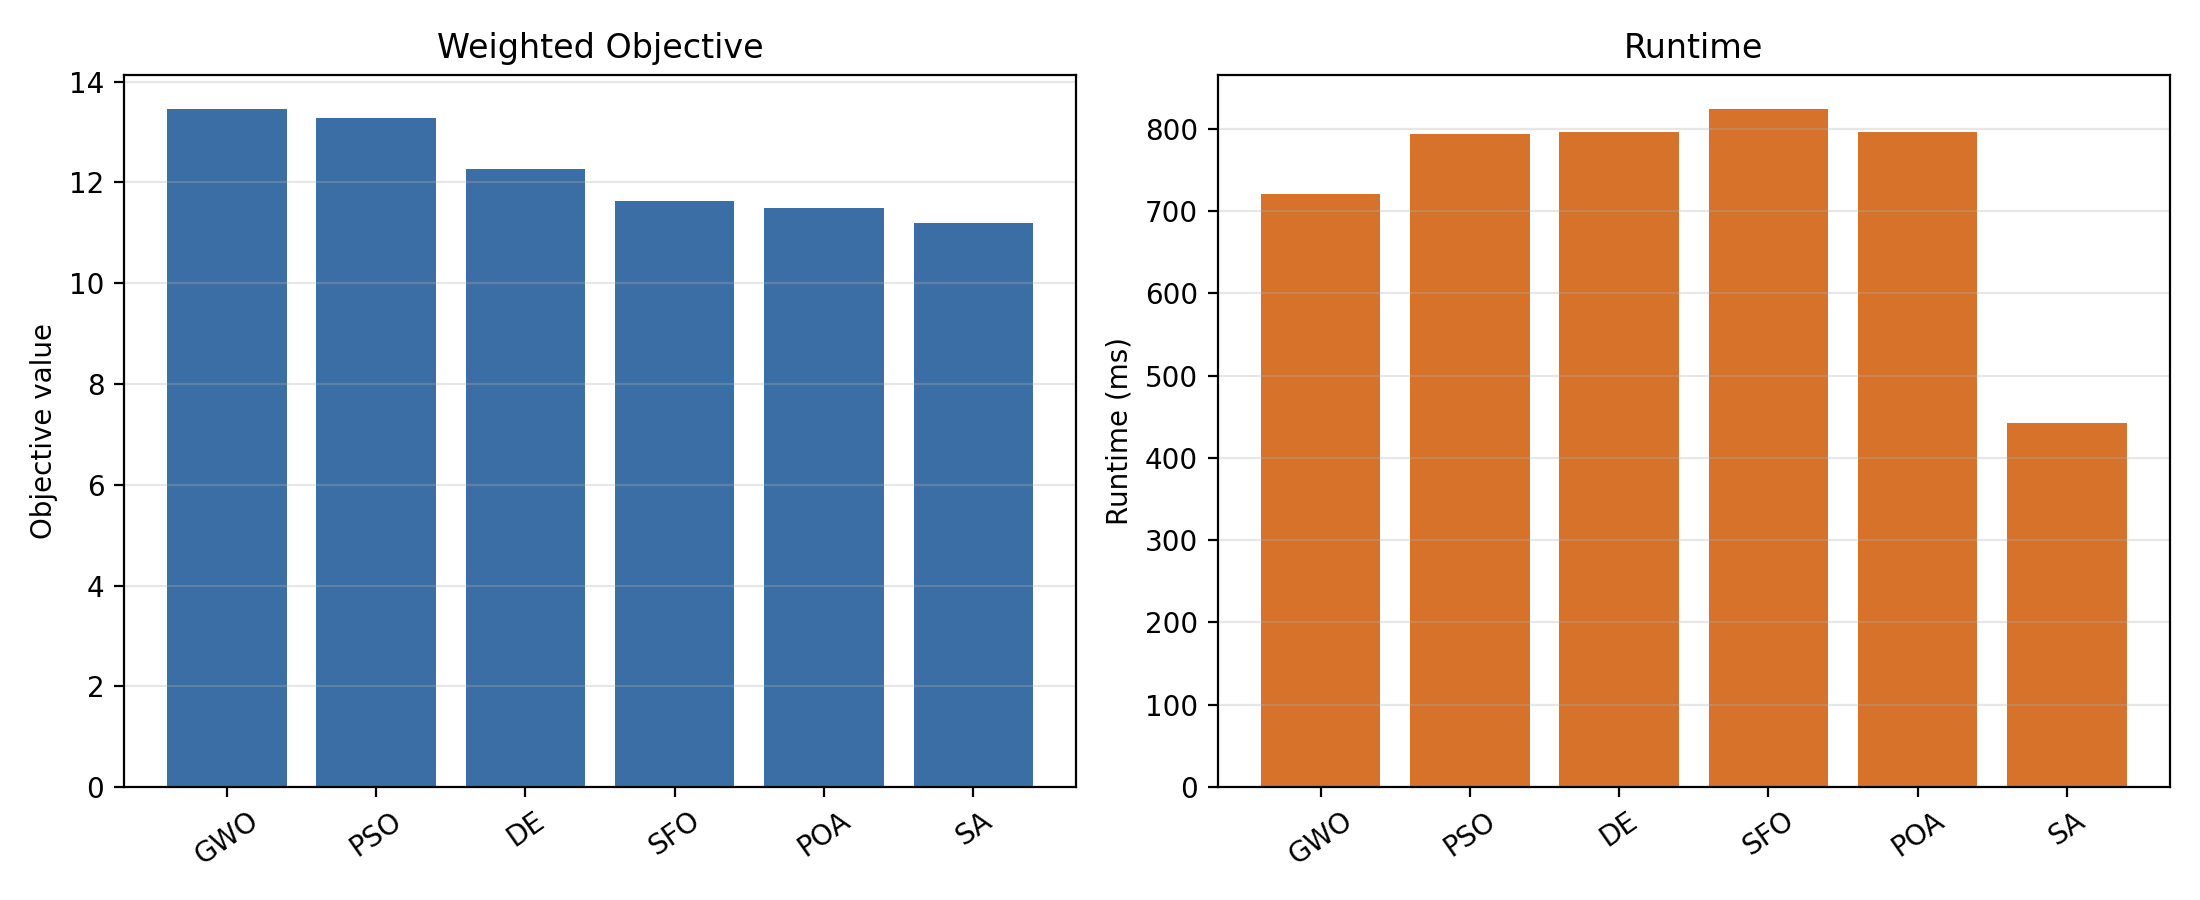
\includegraphics[width=0.82\textwidth]{algorithm_comparison.png}
\caption{Single-snapshot comparison in the default detection-probability mode.}
\label{fig:static}
\end{figure}

\subsection{Dynamic comparison}
The dynamic experiment is more informative than the single snapshot because it shows how the methods behave as the channel changes over time. Across 20 CSI updates, GWO again has the highest mean score (9.21) and mean $P_d$ (0.526) under the fixed-seed setup. PSO is a close second at 9.13 and 0.501.

\begin{table}[t]
\centering
\caption{Dynamic results over 20 CSI updates.}
\label{tab:dynamic}
\begin{tabular}{lcccc}
\toprule
Solver & Mean score & Mean rate & Mean $P_d$ & Mean runtime (ms) \\
\midrule
GWO & 9.21 & 13.17 & 0.526 & 795.2 \\
PSO & 9.13 & 13.25 & 0.501 & 598.7 \\
POA & 8.47 & 13.48 & 0.346 & 644.0 \\
DE  & 8.21 & 12.58 & 0.383 & 755.9 \\
SFO & 8.02 & 13.36 & 0.268 & 687.4 \\
SA  & 6.98 & 13.17 & 0.080 & 395.6 \\
\bottomrule
\end{tabular}
\end{table}

The dynamic study is also useful for interpretation. SA is the fastest method, but it gives the weakest sensing results by a clear margin. GWO and DE take longer, but they preserve much better sensing quality. For offline design, that extra runtime is acceptable. For a stricter real-time setting, PSO may be the more practical compromise because it is close to GWO but cheaper per update.

Figure~\ref{fig:dynamicbars} and Figure~\ref{fig:traces} show the dynamic summary and the time traces.

\begin{figure}[t]
\centering
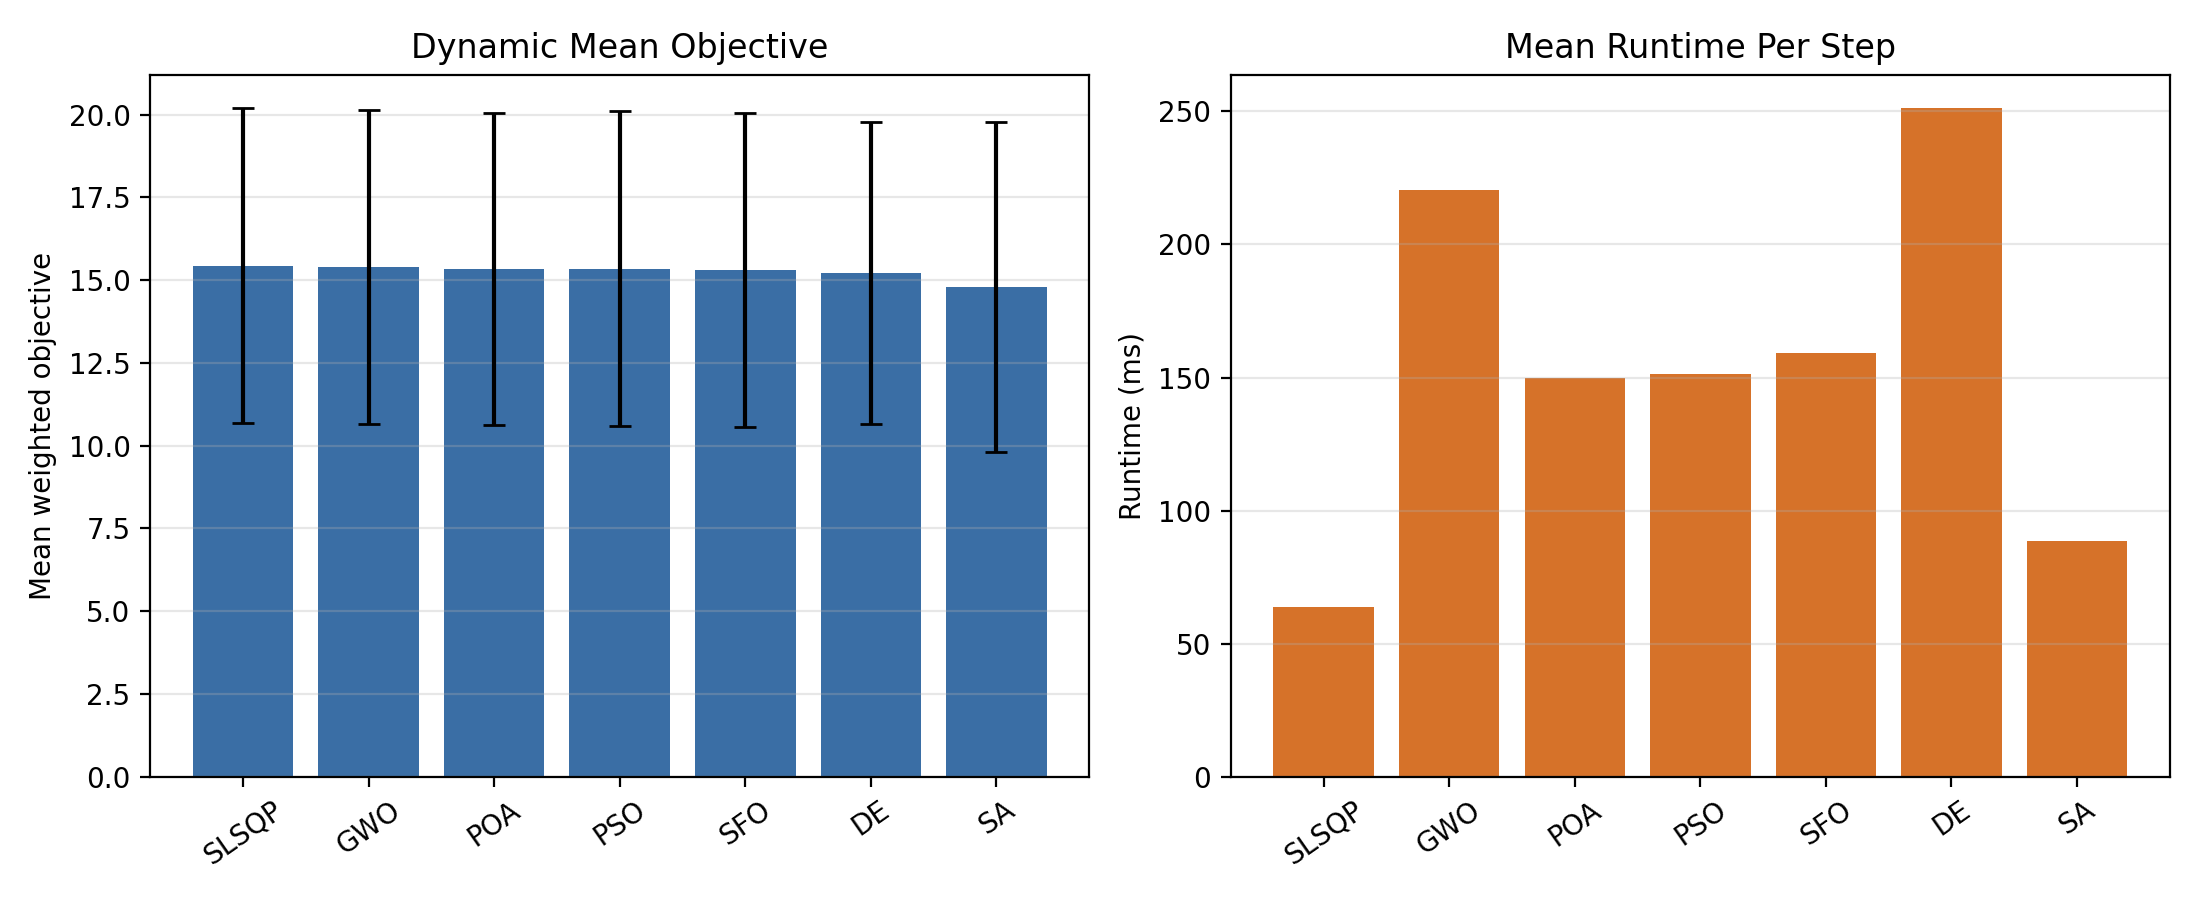
\includegraphics[width=0.82\textwidth]{dynamic_algorithm_comparison.png}
\caption{Mean dynamic performance across the 20 CSI updates.}
\label{fig:dynamicbars}
\end{figure}

\begin{figure}[t]
\centering
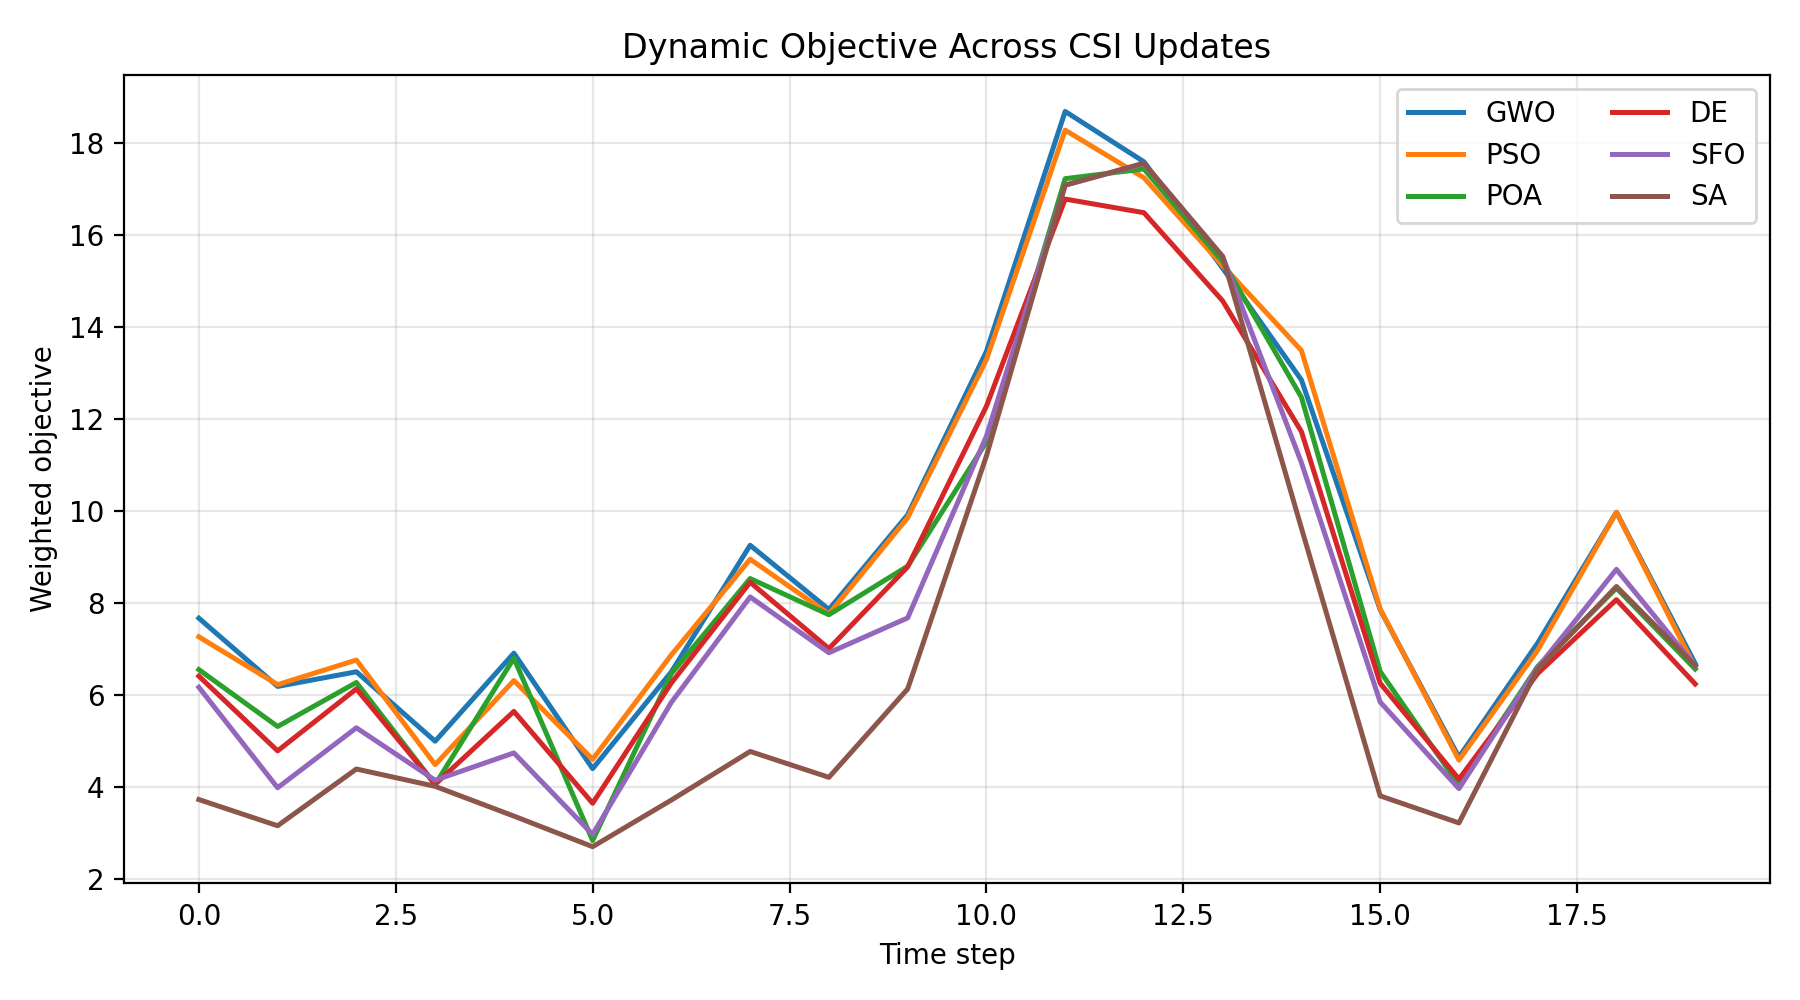
\includegraphics[width=0.82\textwidth]{dynamic_objective_traces.png}
\caption{Objective traces across time for each solver.}
\label{fig:traces}
\end{figure}

\subsection{Tradeoff and Pareto results}
The Pareto study is the clearest place to see the paper's main idea. GWO generated 10 weighted-sum points across $\alpha \in [0,1]$. NSGA-II returned 48 non-dominated solutions, which is useful as a reference front. The two methods are not answering exactly the same question: GWO is searching weighted operating points, while NSGA-II is trying to map out the front more broadly.

\begin{table}[t]
\centering
\caption{Key endpoints in the \texttt{UMi\_NLOS} Pareto study.}
\label{tab:pareto}
\begin{tabular}{lccc}
\toprule
Case & Rate (bps/Hz) & $P_d$ & Comment \\
\midrule
GWO, $\alpha=0$ & 10.70 & 0.892 & sensing-focused end \\
GWO, $\alpha=1$ & 22.76 & 0.212 & rate-focused end \\
Equal power & 20.97 & 0.139 & simple baseline \\
Water-filling & 22.50 & 0.114 & rate-first baseline \\
\bottomrule
\end{tabular}
\end{table}

At the sensing-focused end, GWO reaches $P_d=0.892$. At the rate-focused end, it still keeps $P_d=0.212$ while reaching 22.76 bps/Hz. That wide span matters because it shows that the added waveform variable is not redundant. The optimizer is using it to move between different parts of the tradeoff curve.

The baselines make the point even clearer. Equal power is decent for rate but weak for detection. Water-filling is the best rate-only baseline, but it is even weaker in $P_d$. So a classical power-only strategy is not enough if detection probability is the main sensing goal.

\begin{figure}[t]
\centering
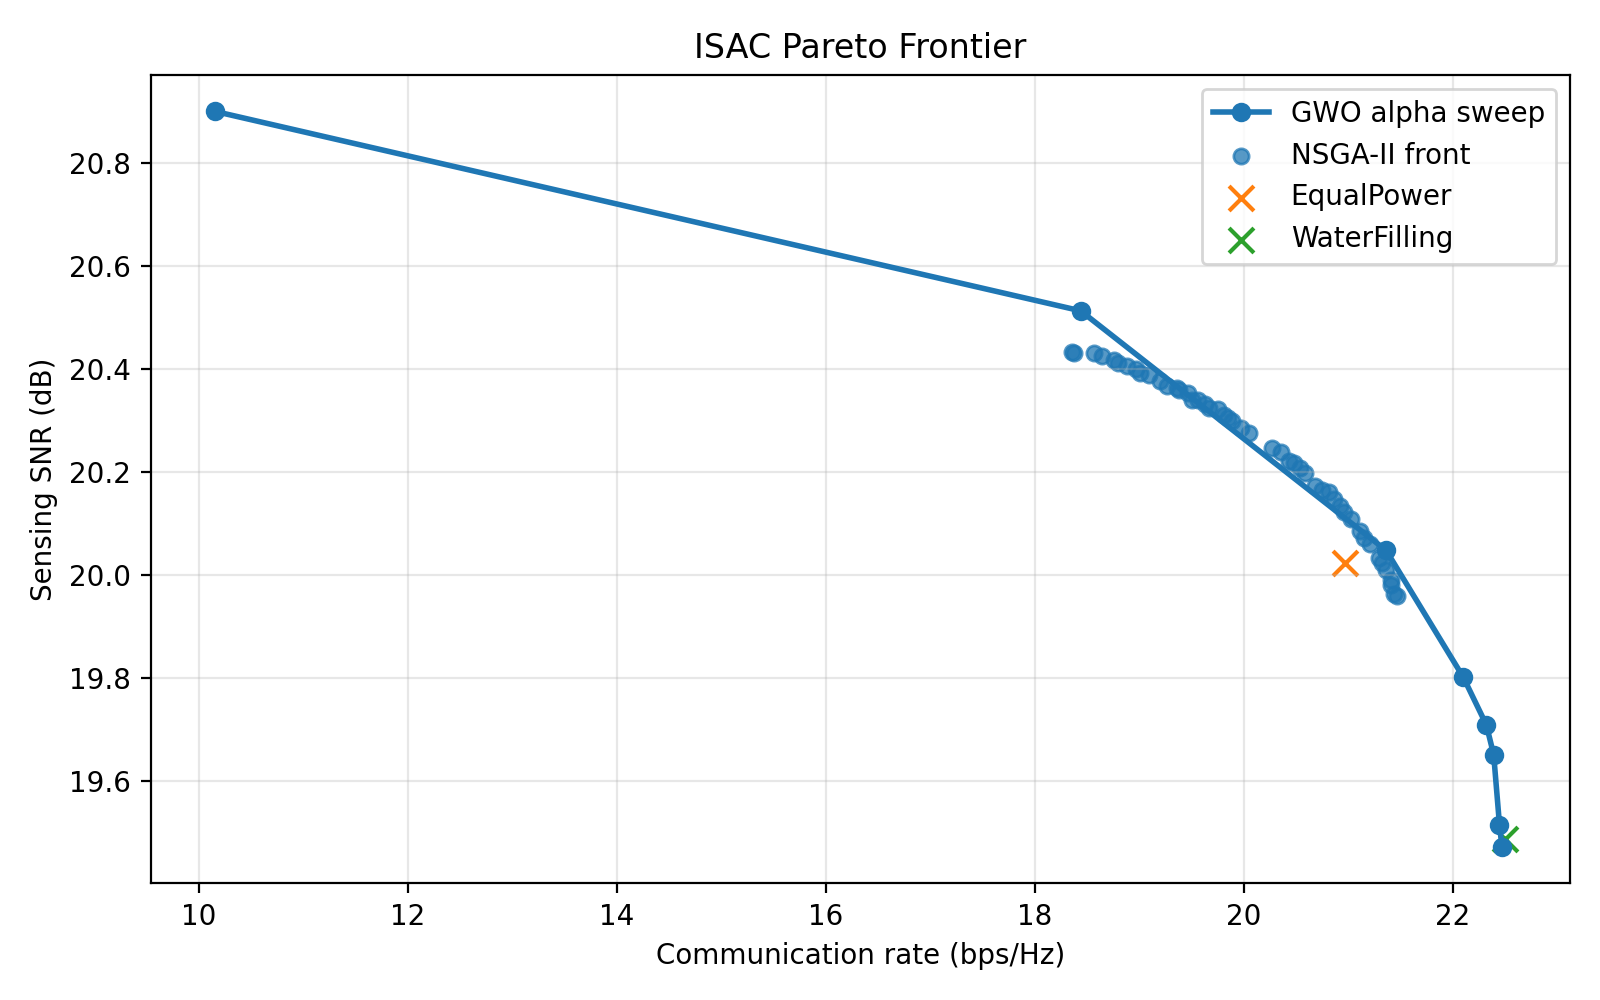
\includegraphics[width=0.82\textwidth]{pareto_front.png}
\caption{Pareto-style view of the \texttt{UMi\_NLOS} snapshot.}
\label{fig:pareto}
\end{figure}

\subsection{Waveform behavior}
The optimized waveform profiles in the saved results are not flat (Figure~\ref{fig:waveforms}). That is important because it shows the waveform variable is doing real work rather than acting as a duplicate of the power vector. In practical terms, the solution places more weight on some subcarriers than others, and that helps it balance detection and communication better than a flat profile. The sensing-focused solution ($\alpha=0$) becomes sharply concentrated, while the rate-focused solution ($\alpha=1$) is closer to flat but still non-uniform.

The waveform variable should be read as a normalized spectral shaping profile, not as a full physical beamforming design. That choice keeps the model simple, but it is still enough to show that waveform shaping changes the result.

\begin{figure}[t]
\centering
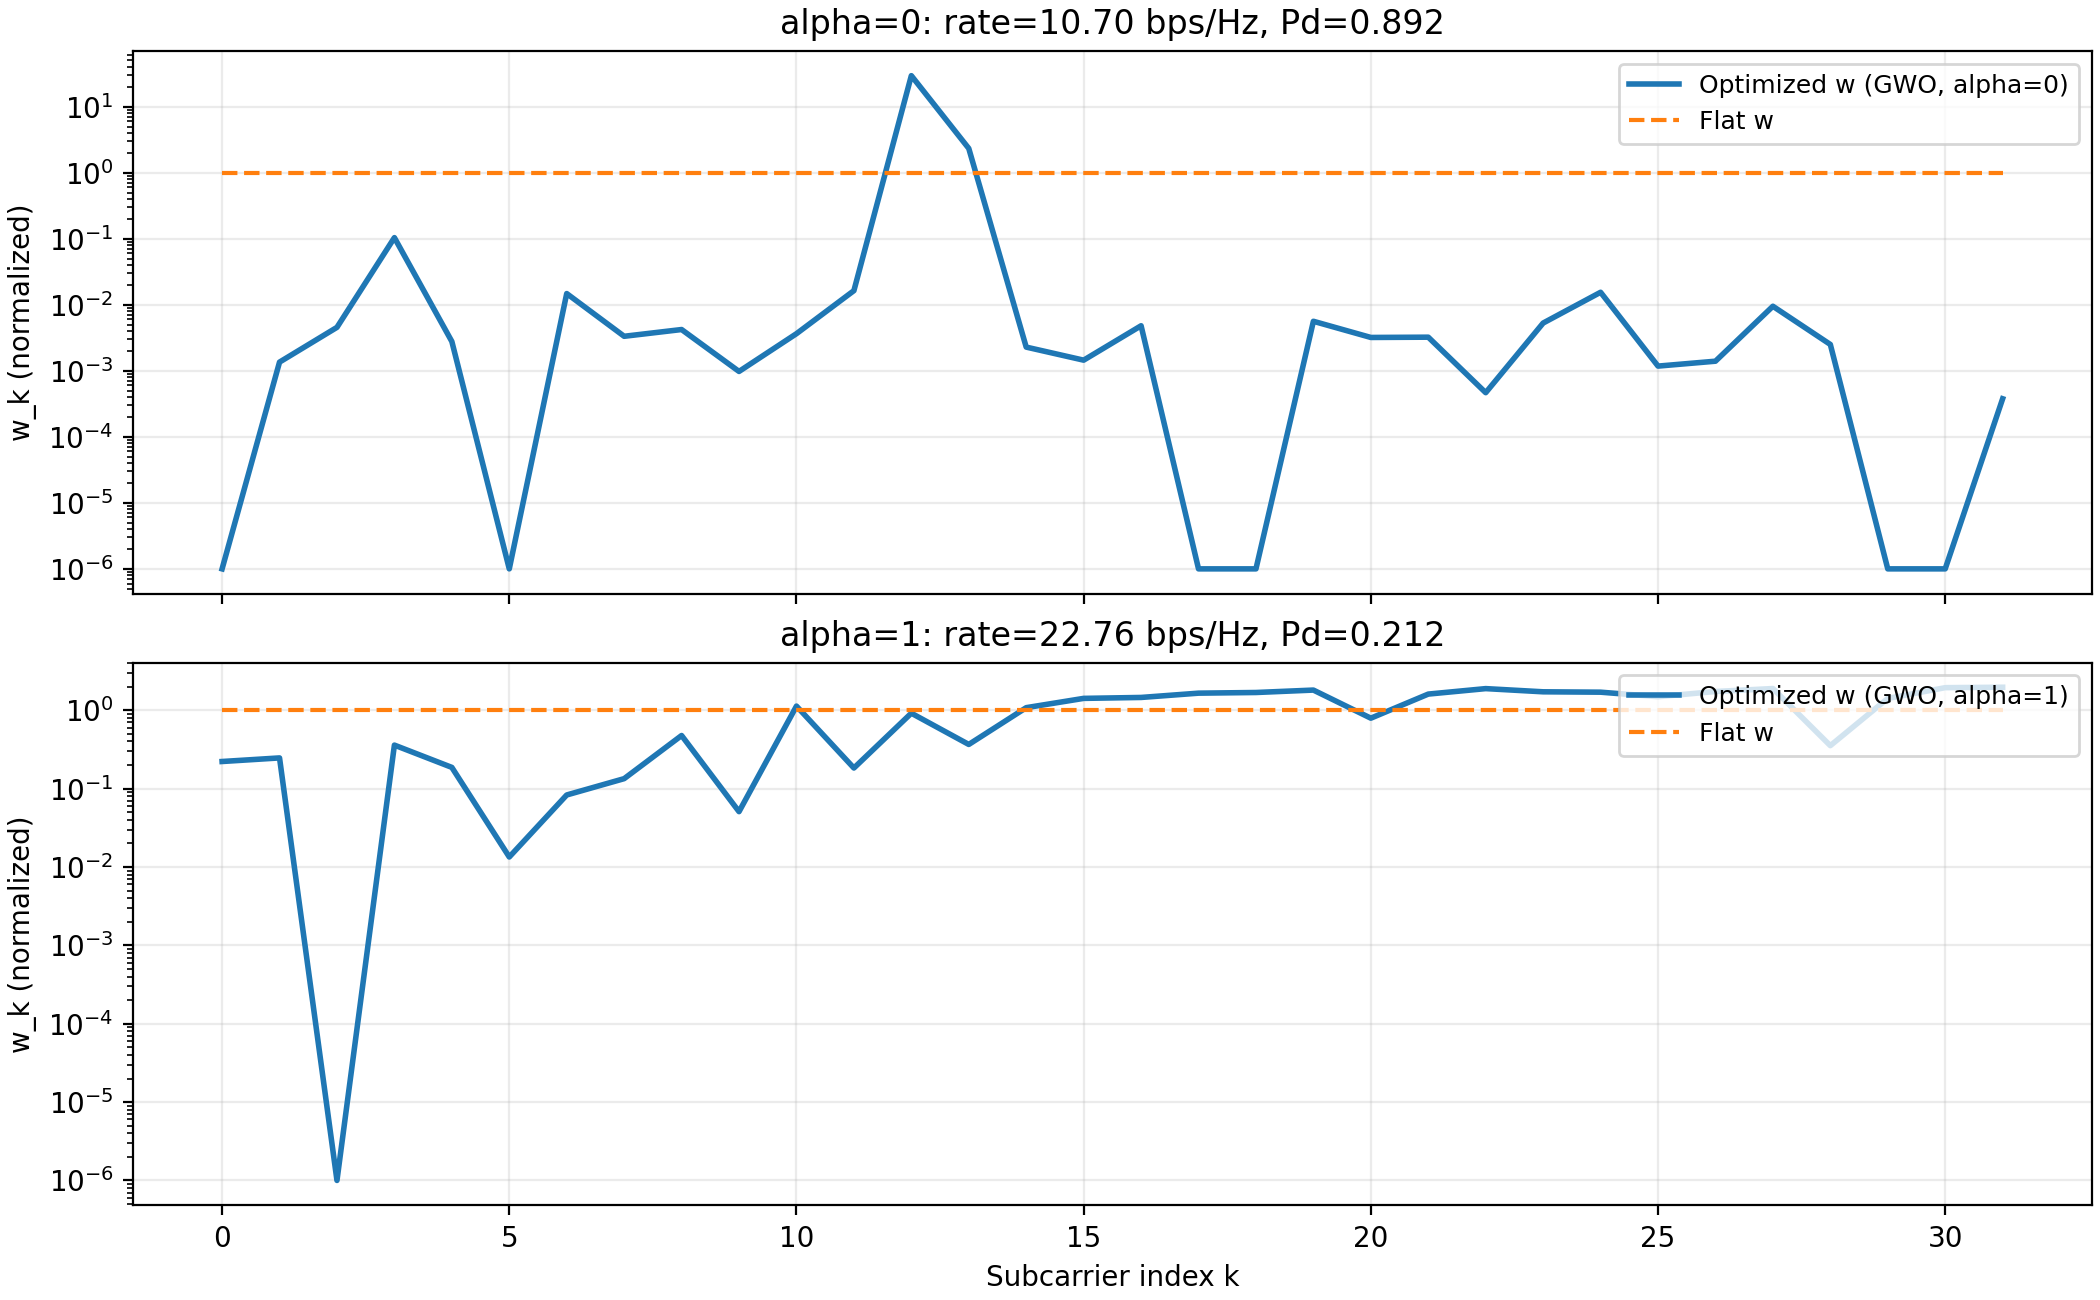
\includegraphics[width=0.82\textwidth]{waveform_profiles.png}
\caption{Example optimized waveform profiles for GWO at the sensing-focused end ($\alpha=0$) and the rate-focused end ($\alpha=1$), compared with a flat profile.}
\label{fig:waveforms}
\end{figure}

\subsection{What the results say}
Taken together, the experiments support three careful conclusions:
\begin{enumerate}
  \item \textbf{GWO and PSO perform comparably under the fixed-seed protocol.} GWO is slightly ahead on the reported weighted score in both the static and dynamic comparisons, but the gap is small and should be read as an indicative ranking rather than a statistically proven win.
  \item \textbf{PSO is a strong alternative when runtime matters.} It matches GWO closely on the combined score and can slightly exceed it on snapshot $P_d$, while tending to be faster in the dynamic study.
  \item \textbf{Waveform co-optimization matters.} The non-flat waveform profiles and the wider tradeoff range show that the added variable changes the design space in a meaningful way.
\end{enumerate}

These are benchmark conclusions, not universal claims. They hold for the \texttt{UMi\_NLOS} scenario and the chosen settings.

\section{Limitations and Future Work}
This study is intentionally simple in a few places. Those simplifications do not make the results invalid, but they do limit how far the claims should be stretched.

\begin{itemize}
  \item The static comparison uses one representative snapshot rather than 50--100 Monte Carlo drops.
  \item Each solver is reported for a single fixed random seed (Table~\ref{tab:settings}); therefore small score differences should not be interpreted as statistically significant.
  \item The sensing branch is a single-target return model and does not include clutter or multi-target structure.
  \item The detection-probability mapping uses an effective integration parameter that is useful for comparison but not derived from a full detector model.
  \item The paper does not include matched-filter, Neyman--Pearson, or MMSE beamforming baselines.
  \item The algorithms are compared as search methods for the same weighted objective, not as complete sensing receivers.
\end{itemize}

These points should be stated clearly in the manuscript. Doing so does not weaken the paper; it makes it more credible. The natural future steps are Monte Carlo averaging, more detailed sensing physics, and additional baselines that operate on the detector side rather than only on the allocation side.

\section{Conclusion}
This paper presents a small but focused ISAC case study for the \texttt{UMi\_NLOS} scenario. The main message is that detection probability and waveform shaping should be treated as first-class design variables if the sensing task is detection-oriented. Under the fixed-seed protocol used here, GWO has a slight edge on the weighted objective and PSO is a close and often faster alternative; power-only baselines such as water-filling remain strong on rate but weak on detection. The Pareto endpoints and the non-flat optimized waveform profiles support the practical value of detection-aware waveform co-optimization.

\clearpage
\begin{thebibliography}{99}
\bibitem{liu2022isacsurvey}
Liu, A., Huang, Z., Li, M., Wan, Y., Li, W., Han, X., Liu, C., Du, R., Tan, D.K.P., Lu, J., Shen, Y., Colone, F., Chetty, K.: A survey on fundamental limits of integrated sensing and communication. IEEE Commun. Surv. Tutor. \textbf{24}(2), 994--1034 (2022)

\bibitem{ouyang2023mi}
Ouyang, C., Liu, Y., Yang, H., Al-Dhahir, N.: Integrated sensing and communications: A mutual information-based framework. IEEE Commun. Mag. \textbf{61}(5), 26--32 (2023)

\bibitem{liyanarachchi2021waveforms}
Liyanaarachchi, S.D., Riihonen, T., Barneto, C.B., Valkama, M.: Optimized waveforms for 5G--6G communication with sensing: Theory, simulations and experiments. IEEE Trans. Wireless Commun. \textbf{20}(12), 8301--8315 (2021)

\bibitem{3gpp38901}
3GPP: Study on channel model for frequencies from 0.5 to 100 GHz. Technical Report TR 38.901, Release 14 and later revisions.

\bibitem{mirjalili2014gwo}
Mirjalili, S., Mirjalili, S.M., Lewis, A.: Grey Wolf Optimizer. Adv. Eng. Softw. \textbf{69}, 46--61 (2014)

\bibitem{kennedy1995pso}
Kennedy, J., Eberhart, R.: Particle swarm optimization. In: Proceedings of ICNN'95, vol.~4, pp.~1942--1948. IEEE (1995)

\bibitem{storn1997de}
Storn, R., Price, K.: Differential evolution: A simple and efficient heuristic for global optimization over continuous spaces. J. Glob. Optim. \textbf{11}(4), 341--359 (1997)

\bibitem{deb2002nsga2}
Deb, K., Pratap, A., Agarwal, S., Meyarivan, T.: A fast and elitist multiobjective genetic algorithm: NSGA-II. IEEE Trans. Evol. Comput. \textbf{6}(2), 182--197 (2002)

\bibitem{kay_detection}
Kay, S.M.: Fundamentals of Statistical Signal Processing, Volume~2: Detection Theory. Prentice Hall, Upper Saddle River (1998)

\bibitem{richards_radar}
Richards, M.A.: Fundamentals of Radar Signal Processing, 2nd edn. McGraw-Hill Education, New York (2014)

\bibitem{cover2006}
Cover, T.M., Thomas, J.A.: Elements of Information Theory, 2nd edn. Wiley, Hoboken (2006)
\end{thebibliography}

\end{document}
